\documentclass[xcolor={dvipsnames,rgb}, aspectratio=169]{beamer}

%%% PACKAGES %%%
\usepackage[T1]{fontenc}
\usepackage{tgheros}

% Metropolis customization
\usetheme[sectionpage=none]{metropolis}
\setbeamercolor{background canvas}{bg=white}
\setbeamercolor{frametitle}{bg = white, fg=black}
\setbeamertemplate{sections/subsections in toc}[square]
\setbeamertemplate{footline}{
   \textcolor{bluepoli}{\rule{\paperwidth}{1pt}}
   \vskip4pt
   \hskip5pt \tiny Introduction to Matlab $|$ Calcoli di Processo dell' Ingegneria
   Chimica \hskip250pt \insertframenumber
   \vskip4pt
}

% color
\usepackage{color}
\usepackage{xcolor}
\usepackage{colortbl}
\definecolor{bluepoli}{cmyk}{0.4,0.1,0,0.4}
\definecolor{mygreen}{RGB}{1, 121,111}
\definecolor{myred}{RGB}{220, 20, 60}
\definecolor{mygreen}{RGB}{28,172,0}
\definecolor{mylilas}{RGB}{170,55,241}
\definecolor{codegreen}{rgb}{0,0.6,0}
\definecolor{codegray}{rgb}{0.5,0.5,0.5}
\definecolor{codepurple}{rgb}{0.58,0,0.82}
\definecolor{backcolour}{rgb}{0.95,0.95,0.92}
\definecolor{lightblue}{rgb}{56, 167, 232}

\colorlet{colorp}{NavyBlue}
\colorlet{colorT}{WildStrawberry}
\colorlet{colork}{OliveGreen}
\colorlet{colorM}{RoyalPurple}
\colorlet{colorNb}{Plum}
\colorlet{colorIs}{black}
\newcommand{\highlight}[2]{\colorbox{#1!17}{$#2$}}
\newcommand{\highlightdark}[2]{\colorbox{#1!47}{$#2$}}

% tikz
\usepackage{tikz}
\usetikzlibrary{positioning}
\usetikzlibrary{backgrounds}
\usetikzlibrary{arrows,shapes}
\usetikzlibrary{tikzmark}
\usetikzlibrary{calc}

% tcolorbox env
% Coloured box for styling theorems, proof, definitions
\usepackage[most]{tcolorbox}

\newtcolorbox{code}[2][]{
    enhanced jigsaw,
    colframe=bluepoli,
    interior hidden, 
    breakable,
    before skip=10pt,
    after skip=10pt
}

% URL and Hyperref
\usepackage{hyperref}
\hypersetup{
    colorlinks=true,
    linkcolor=blue,
    filecolor=magenta,      
    urlcolor=blue,
    pdftitle={Overleaf Example},
    pdfpagemode=FullScreen,
}
\usepackage{url}

% Math stuff
\usepackage{amsmath}
\usepackage{amssymb}
\usepackage{mathtools}
\usepackage{blkarray}
\usepackage{multirow}

% Wrapfig
\usepackage{wrapfig}

% Bibliography
\usepackage[
backend=biber,
style=alphabetic,
sorting=ynt
]{biblatex}
\addbibresource{bibliography.bib}

%%% TITLE %%%
\title{Introduction to MATLAB}
\subtitle{Calcoli di Processo dell' Ingegneria Chimica}
\author[Dinelli, Mehl]{\textbf{Timoteo~Dinelli}, \textbf{Marco~Mehl}}
\institute{
   \inst{} Department of Chemistry, Materials and Chemical Enginering, G. Natta.
   Politecnico di Milano.\\
   email: timoteo.dinelli@polimi.it \\
   email: marco.mehl@polimi.it \\
}
\date{20\textsuperscript{\underline{th}} of September 2024,\\
27\textsuperscript{\underline{th}} of September 2024,\\
3\textsuperscript{\underline{rd}} of October 2024.}


\begin{document}
% external files inclusion
% Double underline
\def\doubleunderline#1{\underline{\underline{#1}}}

% \newcommand{\zm}{%
%    \begin{bmatrix}
%       X_{11} & X_{12} & \cdots & X_{1p} \\
%       X_{12} & X_{22} & \cdots & X_{2p} \\
%       \vdots & \vdots & \tikzmarknode{Is}{\highlight{colorT}{X_{ij}}} & \vdots \\
%       X_{n1} & X_{n2} & \cdots & X_{np} \\
%    \end{bmatrix}%
% }

\makeatletter
\newcommand{\DrawLine}{%
  \begin{tikzpicture}
  \path[use as bounding box] (0,0) -- (\linewidth,0);
  \draw[color=bluepoli,dashed,dash phase=2pt]
        (0-\kvtcb@leftlower-\kvtcb@boxsep,0)--
        (\linewidth+\kvtcb@rightlower+\kvtcb@boxsep,0);
  \end{tikzpicture}%
  }
\makeatother

{%
   \setbeamertemplate{footline}{}
   \begin{frame}{}
      \maketitle
      \begin{tikzpicture}[overlay, remember picture]
         \node[above left=6.5cm and .01cm of current page.south east] {
            
\includegraphics[trim=1cm 1cm 1.5cm 1cm, clip=true, width=6cm]{
               figures/_static/ING_IND_INF.eps
            }
         };
         % \node[above left=7.5cm and 6.5cm of current page.south east] {
         %    
\includegraphics[clip=true, width=3cm]{
         %       figures/_static/crecklogo.png
         %    }
         % };
      \end{tikzpicture}
   \end{frame}
}

\begin{frame}{Contacts and Informations}
   Professor Marco Mehl \\
   \textbf{e-mail}: marco.mehl@polimi.it \\
   \textbf{Ufficio}: Campus Leonardo, Edificio 6, DCMIC “G. Natta” (Sezione Ingegneria
   Chimica) \\
   \vskip 1.5cm
   Ing. Timoteo Dinelli \\
   \textbf{e-mail}: timoteo.dinelli@polimi.it \\
   \textbf{Ufficio}: Campus Leonardo, Edificio 6, DCMIC “G. Natta” (Sezione Ingegneria
   Chimica)
\end{frame}

% \section{Resources}
\begin{frame}{Resources}
   \small \alert{Books}:
   \begin{itemize}
      \item[$\blacktriangleright$]
         \href{http://hdl.handle.net/11311/579545}{\footnotesize G., Buzzi Ferraris;
         Manenti, Flavio. Fundamentals and Linear Algebra for the Chemical Engineer:
         Solving Numerical Problems.} 
      \item[$\blacktriangleright$]
         \href{http://hdl.handle.net/11311/579546}{\footnotesize G., Buzzi Ferraris;
         Manenti, Flavio. Interpolation and Regression Models for the Chemical Engineer:
         Solving Numerical Problems.} 
      \item[$\blacktriangleright$]
         \href{http://hdl.handle.net/11311/663722}{\footnotesize G., Buzzi Ferraris;
         Manenti, Flavio. Nonlinear Systems and Optimization for the Chemical Engineer:
         Solving Numerical Problems.}
      \item[$\blacktriangleright$]
         \href{http://hdl.handle.net/11311/1003033}{\footnotesize G., Buzzi Ferraris;
         Manenti, Flavio. Differential and Differential-Algebraic Systems for the
         Chemical Engineer: Solving Numerical Problems.}
      \item[$\blacktriangleright$]
         \href{https://www.biblio.com/9780199660346}{\footnotesize J. Nathan Kutz.
         Data-Driven Modeling and Scientific Computation.}
   \end{itemize}
\end{frame}

\begin{frame}{}
   \begin{itemize}
      \item[$\blacktriangleright$]
         \href{https://www.amazon.it/Data-Driven-Science-Engineering-Learning-Dynamical/dp/1009098489/ref=asc_df_1009098489/?tag=googshopit-21&linkCode=df0&hvadid=560287860614&hvpos=&hvnetw=g&hvrand=14266207767663986773&hvpone=&hvptwo=&hvqmt=&hvdev=c&hvdvcmdl=&hvlocint=&hvlocphy=1008463&hvtargid=pla-1599460130783&psc=1}{\footnotesize
         Steven L. Brunton; J. Nathan Kutz. Data-Driven Science and Engineering: Machine
         Learning, Dynamical Systems, and Control.}
      \item[$\blacktriangleright$]
         \href{https://link.springer.com/book/10.1007/978-88-470-5644-2}{\footnotesize A.
         Quarteroni; R. Sacco; F. Saleri; P. Gervasio. Matematica Numerica.}
      \item[$\blacktriangleright$]
         \href{https://www.amazon.it/Calcolo-Scientifico-Esercizi-problemi-risolti-dp-8847039525/dp/8847039525/ref=dp_ob_title_bk}{\footnotesize
         A. Quarteroni; F. Saleri; P. Gervasio. Calcolo Scientifico: Esercizi e problemi
         risolti con MATLAB e Octave.}
      \item[$\blacktriangleright$]
         \href{https://www.ibs.it/calcolo-numerico-applicato-libro-davide-manca/e/9788837116972}{\footnotesize
         D. Manca. Calcolo numerico applicato.}
   \end{itemize}
   \vskip 1.cm
   \small \alert{Online Material}:
      \begin{itemize}
         \item[$\blacktriangleright$]
            \href{https://ocw.mit.edu/courses/10-34-numerical-methods-applied-to-chemical-engineering-fall-2015/pages/syllabus/}{\footnotesize
            Numerical Methods applied to chemical engineering (MIT).}
         \item[$\blacktriangleright$]
            \href{https://github.com/Titodinelli/Calcoli-di-Processo-dell-Ingegneria-Chimica}{\footnotesize
            GitHub repository of the practical sessions.}
         \item[$\blacktriangleright$]
            \href{https://it.mathworks.com/help/matlab/getting-started-with-matlab.html}{\footnotesize
            Matlab online tutorial and documentation.}
    \end{itemize}
\end{frame}

% \begin{frame}
%    \frametitle{Table of Contents}
%    \hypersetup{linkcolor=black}{\tableofcontents}
% \end{frame}
\begin{frame}
\frametitle{Table of Contents}
   \begin{columns}[t] % 't' allinea le colonne in alto
      \begin{column}{0.5\textwidth}
         \hypersetup{linkcolor=black}{\tableofcontents[sections={1-3}]}
      \end{column}
      \begin{column}{0.5\textwidth}
         \hypersetup{linkcolor=black}{\tableofcontents[sections={4-5}]}
      \end{column}
   \end{columns}
\end{frame}

\section{Introduction}
\subsection{What is programming?}
\begin{frame}{What is programming?}
\small{
\begin{itemize}
   \item[$\blacktriangleright$] The most simple answer is: ``Programming is the
      \underline{\textbf{act}} or activity of writing computer programs.''. In a
      more general way programming or coding is the act of writing a computer program.

   \item[$\blacktriangleright$] A \underline{\textbf{computer program}} is a sequence of
      instructions that a computer is able to execute.

   \item[$\blacktriangleright$] \underline{\textbf{Computer}} in the definition above is
      any device that is capable of processing code. This could be smartphones, ATMs, the
      Raspberry Pi, Servers to name a few.
\end{itemize}

Remember, every time we use smart devices, some code is running in the background.
Moving a mouse pointer from one part of your computer screen to the other may seem
like a simple task, but in reality, so many lines of code just ran. An act as simple
as typing letters into Google Docs leads to lines of code being executed in the
background. It’s all code everywhere.}
\end{frame}

\subsection{The Natural Language of Computers}
\begin{frame}{The Natural Language of Computers}
\begin{columns}
   \begin{column}{0.5\textwidth}
      \begin{figure}
         \centering
         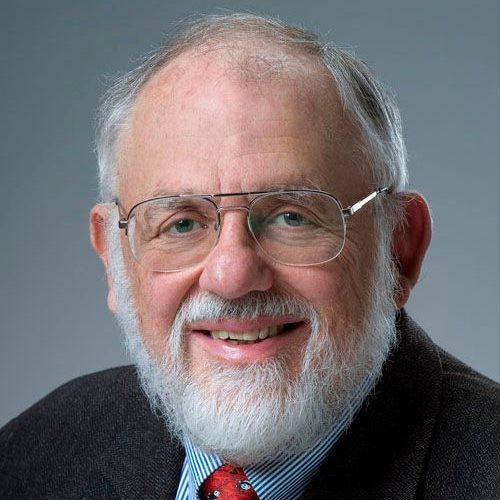
\includegraphics[width=0.85\textwidth]{figures/cleve_moler.jpg}
         % \label{fig:clevmol}
         \caption{Cleve Barry Moler}
      \end{figure}
   \end{column}

   \begin{column}{0.5\textwidth}
      \small{The \underline{\textbf{only}} language understood by a computer is the machine
      language. A very long list of 0 and 1. However it is a little bit inconvenient
      to write a series of zeros and ones. So (very smart) people, like the one in the
      picture, invented what are called programming languages (C/C++, Fortran, python,
      julia, MATLAB, ...).

      \alert{\textbf{N.B.}} Computers aren't very smart, the instructions
      need to be very precise! Telling a computer what you want it to do is sometimes
      hard because you have to explain things very carefully and precisely.}
   \end{column}
\end{columns}
\end{frame}

\section{First Steps with MATLAB}
\begin{frame}{MATLAB}
\begin{figure}
   \centering
   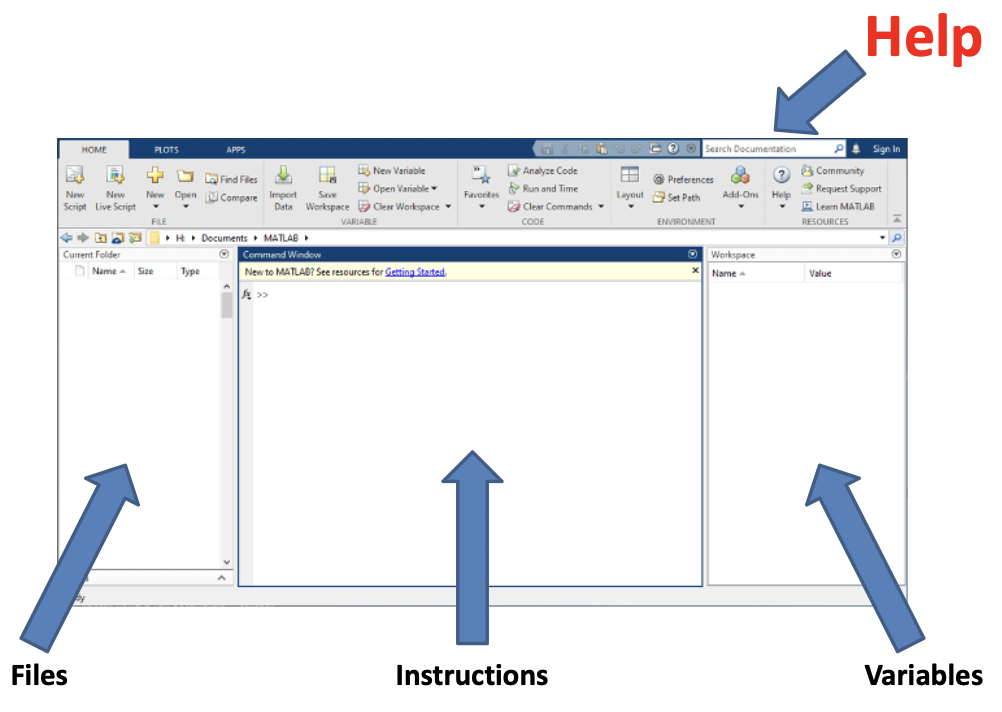
\includegraphics[width=0.7\textwidth]{Figures/MATLAB-2.png}
\end{figure}
\end{frame}

\begin{frame}{What can a Computer handle?}
\begin{itemize}
   \item[$\blacktriangleright$] MATLAB deals with numbers, arrays of numbers, characters,
      strings.
   \item[$\blacktriangleright$] Numbers can be of different types: signed and unsigned
      integers, and single-precision and double-precision floating-point numbers.
   \item[$\blacktriangleright$] When we set a variable value it gets stored as a series
      of 0 and 1 in a memory slot whose size depends on the type of variable (i.e.,
      single-precision floating point numbers take 32 bits, or 4 bytes of memory, double
      precision 64 bit, or 8 bytes).
   \item[$\blacktriangleright$] By default, MATLAB store all values as double-precision
      floating point.
\end{itemize}
\end{frame}

\subsection{Variables}
\begin{frame}{Area of a cylinder}
\large \textcolor{mylilas}{Let's compute the area of a cylinder given the diameter D = 20 cm
and height h = 50 cm}.

\begin{tcolorbox}[colback=white,colframe=bluepoli,sidebyside]
   \vskip -2.cm
   \textcolor{mygreen}{Command window}\\
      $>>$ D = 0.2 \textcolor{codegreen}{ \% m} \\
      $>>$ h = 0.5 \textcolor{codegreen}{ \% m} \\
      $>>$ perimeter = pi * D\\
      $>>$ Area = perimeter * h
   \tcblower
   \textcolor{mygreen}{Workspace} \\
      \small $\rightarrow$ Generate variable D and assign value of 0.2\\
      $\rightarrow$ Generate variable h and assign value of 0.5\\
      $\rightarrow$ Generate variable perimeter and assign the result of the operation.\\
      $\rightarrow$ Generate variable Area and assign the result of the operation.\\
\end{tcolorbox}
\end{frame}

\begin{frame}{Source code: scripts and functions in MATLAB}
Scripts are m-files (text format) containing MATLAB statements. MATLAB ``functions'' are
another type of m-file. The biggest difference between scripts and functions is that
functions have input and output parameters. Script files can only operate on the
variables that are ``hard-coded'' into their m-file.

% \vspace{-10pt}
\begin{columns}[T]%beamer
\column{0.45\textwidth}
   \begin{tcolorbox}[colback=white,colframe=bluepoli]
      $>>$ D = 0.2 \color{codegreen} \% m \color{black} \\
      $>>$ h = 0.5 \color{codegreen} \% m \color{black}\\
      $>>$ perimeter = pi * D\\
      $>>$ Area = perimeter * h
      \tcblower
      ans = 0.3142
   \end{tcolorbox}
\column{0.55\textwidth}
   \begin{tcolorbox}[colback=white,colframe=bluepoli]
      \color{blue} function \color{black}
      Area = ComputeArea(D, h) \\
      perimeter = pi * D; \\
      Area = perimeter * h;\\
      \color{blue} end
      \tcblower
      $>>$ ComputeArea(0.2, 0.5) \\
      $>>$ ans = 0.3142
   \end{tcolorbox}
\end{columns}
\end{frame}

\begin{frame}{Variables names}
\begin{itemize}
   \item[$\blacktriangleright$] MATLAB is case sensitive! \textbf{Pippo $\neq$ pippo}
   \item[$\blacktriangleright$] Variables name should be self explanatory, so prefer
      \textbf{distance, radius, ...} than \textbf{a, b, ...}
   \item[$\blacktriangleright$] When possible \underline{\textbf{use}} the camel case
      notation to make stuff easier to read. \textbf{PipeLength, GasTemperature, ...}.
\end{itemize}
\end{frame}

\subsection{Arrays and Matrices}
\begin{frame}{Arrays and Matrices}
\vskip -.5cm
\begin{itemize}
   \item[$\blacktriangleright$] In MATLAB \textbf{arrays} are defined as:
      \begin{tcolorbox}[colback=white,colframe=bluepoli]
         $>>$ v = [5 13 97 31 98] \\
         v = \\
         \hspace{3em} 5 \hspace{3em} 13 \hspace{3em} 97 \hspace{3em} 31 \hspace{3em} 98
      \end{tcolorbox}
   \item[$\blacktriangleright$] \textbf{Matrices} can be defined as a set of stacked arrays separated with ; 
   \begin{tcolorbox}[colback=white,colframe=bluepoli]
      $>>$ M = [5 13 97; 31 98 36; 11 9 20] \\
      M = \\
      \hspace{3em} 5 \hspace{3em} 13 \hspace{3em} 97 \\
      \hspace{3em} 31 \hspace{3em} 98 \hspace{3em} 36 \\
      \hspace{3em} 11 \hspace{3em} 9 \hspace{3em} 20
   \end{tcolorbox}
\end{itemize}
\end{frame}

\begin{frame}{}
\begin{itemize}
\item[$\blacktriangleright$] Elements can be accessed using their index (indices in
   MATLAB starts from 1)
   \begin{tcolorbox}[colback=white,colframe=bluepoli]
      $>>$ v(1) \\
      ans = 5
   \end{tcolorbox}

   \begin{tcolorbox}[colback=white,colframe=bluepoli]
      $>>$ M(2,1) \color{codegreen} \% (row number, column number) \\
      \color{black}
      ans = 31
   \end{tcolorbox}
\end{itemize}
\end{frame}

\begin{frame}{Creating arrays and matrices}
\begin{itemize}
    \item[$\blacktriangleright$] Create a matrix of zeros or ones:
    \begin{columns}[T]%beamer
    \column{0.5\textwidth}
        \begin{tcolorbox}[colback=white,colframe=bluepoli]
        $>>$ A = zeros(3,2) \\
        A = \\
        \hspace{3em} 0 \hspace{3em} 0 \\
        \hspace{3em} 0 \hspace{3em} 0 \\
        \hspace{3em} 0 \hspace{3em} 0
        \end{tcolorbox}
    \column{0.5\textwidth}
        \begin{tcolorbox}[colback=white,colframe=bluepoli]
        $>>$ A = ones(2,3) \\
        A = \\
        \hspace{3em} 1 \hspace{3em} 1 \hspace{3em} 1 \\
        \hspace{3em} 1 \hspace{3em} 1 \hspace{3em} 1 \\
        \end{tcolorbox}
    \end{columns}
\end{itemize}
\end{frame}

\begin{frame}{}
\begin{itemize}
   \item[$\blacktriangleright$] Create a vector of n equally spaced elements:
      \begin{tcolorbox}[colback=white,colframe=bluepoli]
         $>>$ v1 = [1:2:11] \color{codegreen}\% Parenthesis can be omitted\\
         \color{black}
         v1 = \hspace{3em} 1 \hspace{3em} 3 \hspace{3em} 5 \hspace{3em} 7 \hspace{3em} 9 \hspace{3em} 11
         \tcblower
         $>>$ v2 = [1:3:11] \color{codegreen}\% Parenthesis can be omitted\\
         \color{black}
         v2 = \hspace{3em} 1 \hspace{3em} 4 \hspace{3em} 7 \hspace{3em} 10
         \color{codegreen} \% be careful! \DrawLine \\
         \color{black}
         $>>$ v3 = linspace(1,10,6) \color{codegreen} \% Parenthesis can NOT be omitted!\\
         \color{black}
         v3 = \hspace{3em} 1.0 \hspace{3em} 2.8 \hspace{3em} 4.6 \hspace{3em} 6.4 \hspace{3em} 8.2 \hspace{3em} 10.0
      \end{tcolorbox}
\end{itemize}
\end{frame}

\begin{frame}{Operations with arrays and matrices}
\begin{columns}
\column{0.5\textwidth}
\begin{itemize}
   \vspace{-10pt}
   \item[$\blacktriangleright$] Size of a matrix:
   \begin{tcolorbox}[colback=white,colframe=bluepoli]
      $>>$ M = [1 2 3; 4 5 6] \\
      $>>$ size(M)
      \tcblower
      ans = 2 3
   \end{tcolorbox}

   \vspace{-5pt}
   \item[$\blacktriangleright$] Copying a matrix:
   \begin{tcolorbox}[colback=white,colframe=bluepoli]
      $>>$ A = M 
      \tcblower
      A = \\
      \hspace{3em} 1 \hspace{3em} 2 \hspace{3em} 3 \\
      \hspace{3em} 4 \hspace{3em} 5 \hspace{3em} 6
   \end{tcolorbox}
\end{itemize}
\column{0.5\textwidth}
\begin{itemize}
   \vspace{-10pt}
   \item[$\blacktriangleright$] Copying a line or a column of a matrix:
   \begin{tcolorbox}[colback=white,colframe=bluepoli]
      $>>$ v = M(1,:) 
      \tcblower
      v = \\
      \hspace{3em} 1 \hspace{3em} 2 \hspace{3em} 3
   \end{tcolorbox}

   \item[$\blacktriangleright$] Size of an array:
   \begin{tcolorbox}[colback=white,colframe=bluepoli]
      $>>$ size(v)
      ans = 1 3
      \tcblower
      $>>$ length(v)\\
      ans = 3
   \end{tcolorbox}
\end{itemize}
\end{columns}
\end{frame}

\begin{frame}{}
\begin{columns}
\column{0.5\textwidth}
\begin{itemize}
   \item[$\blacktriangleright$] Matrix transposition:
   \begin{tcolorbox}[colback=white,colframe=bluepoli]
      $>>$ C = B'
      \tcblower
      C = \\
      \hspace{3em} 1 \hspace{3em} 4 \\
      \hspace{3em} 2 \hspace{3em} 5 \\
      \hspace{3em} 3 \hspace{3em} 6 
   \end{tcolorbox}

   \vspace{-10pt}
   \item[$\blacktriangleright$] Element wise multiplication:
   \begin{tcolorbox}[colback=white,colframe=bluepoli]
      $>>$ M .* M
      \tcblower
      ans = \\
      \hspace{3em} 1 \hspace{3em} 4  \hspace{3em} 9\\
      \hspace{3em} 16 \hspace{3em} 25 \hspace{3em} 36
   \end{tcolorbox}
\end{itemize}

\vspace{-10pt}
\column{0.5\textwidth}
   \begin{itemize}
      \item[$\blacktriangleright$] Matrix multiplication:
      \begin{tcolorbox}[colback=white,colframe=bluepoli]
         $>>$ M * B
         \tcblower
         \textcolor{red}{\small{Error using * Inner matrices dimensions must agree.}}
         \DrawLine \\
         $>>$ M * C \\
         \DrawLine \\
         ans = \\
         14 \hspace{3em}32 \\
         32 \hspace{3em}77 \\
         \DrawLine \\
         \textcolor{codegreen}{size(M) = 2 3; size(C) =  3 2}
      \end{tcolorbox}
   \end{itemize}
\end{columns}
\end{frame}

%%%%%%%%%%%%%%% PART 2
{%
   \setbeamertemplate{footline}{}
   \begin{frame}[standout]
      Loops and conditional statements
   \end{frame}
}

\section{Loops}
\subsection{For}
\begin{frame}{\textcolor{blue}{for} loop}
\begin{itemize}
   \item[$\blacktriangleright$] The \textbf{for} loop repeats a series of instructions a
      \alert{fixed number of times}.
   \begin{tcolorbox}[colback=white,colframe=bluepoli]
      $>>$ \textcolor{blue}{for} i = \textcolor{red}{1:10}\\
      $>>$ \hspace{1em}paperino(i) = i \\
      $>>$ \textcolor{blue}{end}
      \tcblower
      paperino = 1 \\
      paperino = 1 2\\
      paperino = 1 2 3\\
      ... \\
      paperino = 1 2 3 4 5 6 7 8 9\\
      paperino = 1 2 3 4 5 6 7 8 9 10
   \end{tcolorbox}
\end{itemize}
\end{frame}

\begin{frame}{}
\begin{itemize}
   \item[$\blacktriangleright$] The index of the \textbf{for} loop can be changed by an
      \alert{arbitrary increment}:
   \begin{tcolorbox}[colback=white,colframe=bluepoli]
      $>>$ \textcolor{blue}{for} i = \textcolor{red}{10:-1:1}\\
      $>>$ \hspace{1em}pluto(i) = i\\
      $>>$ \textcolor{blue}{end}
      \tcblower
      pluto = 0 0 0 0 0 0 0 0 0 10 \\
      pluto = 0 0 0 0 0 0 0 0 9 10 \\
      pluto = 0 0 0 0 0 0 0 8 9 10 \\
      ... \\
      pluto = 0 2 3 4 5 6 7 8 9 10 \\
      pluto = 1 2 3 4 5 6 7 8 9 10 \\
   \end{tcolorbox}
\end{itemize}
\end{frame}

\begin{frame}{Examples}
\begin{itemize}
   \item[$\blacktriangleright$] Sum the first hundred natural numbers.
      \begin{equation*}
         \sum_{i = 1}^{100} i = ?
      \end{equation*}
   \item[$\blacktriangleright$] Sum hundred times one.
      \begin{equation*}
         \sum_{i=1}^{100} 1 = ?
      \end{equation*}
   \begin{tcolorbox}[colback=white,colframe=bluepoli,sidebyside]
      $>>$ sum = 0; \\
      $>>$ \textcolor{blue}{for} i = \textcolor{red}{1:100}\\
      $>>$ \hspace{1em}sum = sum + i;\\
      $>>$ \textcolor{blue}{end}\\
      $>>$ disp(sum);
      \tcblower
      $>>$ sum = 0; \\
      $>>$ \textcolor{blue}{for} i = \textcolor{red}{1:100}\\
      $>>$ \hspace{1em}sum += 1;\\
      $>>$ \textcolor{blue}{end}\\
      $>>$ disp(sum);
    \end{tcolorbox}
\end{itemize}
\end{frame}

\subsection{While}
\begin{frame}{\textcolor{blue}{while}}
\vspace{-10pt}
\begin{itemize}
    \item[$\blacktriangleright$] The \textbf{while} loop repeats a series of instructions
       \alert{until a condition is TRUE}.
    \item[$\blacktriangleright$] N.B. pay attention with the while loop it can run till
       infinite, \alert{handle with care}.
\end{itemize}
\begin{tcolorbox}[colback=white,colframe=bluepoli]
   $>>$ sum = 0; \\
   $>>$ \textcolor{blue}{while} (sum $<$ 325)\\
   $>>$ \hspace{1em}token = token + 1\\
   $>>$ \hspace{1em}sum = sum + token; \\
   $>>$ \textcolor{blue}{end}\\
   disp([''Iteration number: '', num2str(token)]); \\
   disp([''Sum is equal to:  '', num2str(sum)]); 
   \tcblower
   Iteration number: 25 \\
   Sum is equal to: 325
\end{tcolorbox}
\end{frame}

\section{Conditional statements}
\subsection{If, else if, else}
\begin{frame}{IF Statement}
\begin{itemize}
   \item[$\blacktriangleright$] The \textcolor{blue}{\textbf{IF}} statement executes a
      series of instructions only \textcolor{blue}{\textbf{IF}} a condition is TRUE:
\end{itemize}

\begin{columns}
\column{0.5\textwidth}
   \begin{tcolorbox}[colback=white,colframe=bluepoli]
      \textcolor{blue}{if} (condition)\\
      ... instructions\\
      \textcolor{blue}{elseif} (condition)\\
      ... instructions \\
      \textcolor{blue}{elseif} (condition)\\
      ... instructions \\
      \textcolor{blue}{else}\\
      ... instructions \\
      \textcolor{blue}{end}
   \end{tcolorbox}
\column{0.5\textwidth}
   \begin{tcolorbox}[colback=white,colframe=bluepoli]
      \textcolor{mylilas}{Example: Write a simple script to compute the absolute value of
      a number.}\\
      $>>$ x = 35\\
      $>>$ \textcolor{blue}{if} (x$\ge$0)\\
      $>>$ \hspace{1em}abs = x;\\
      $>>$ \textcolor{blue}{else}\\
      $>>$ \hspace{1em}abs = -x\\
      $>>$ \textcolor{blue}{end}
   \end{tcolorbox}
\end{columns}
\end{frame}

\section{Useful functions}
\begin{frame}{Useful Functions}
\begin{itemize}
   \item[$\blacktriangleright$] \textbf{clc}: clear the screen of the command window.
   \item[$\blacktriangleright$] \textbf{clear / clear all}: erase all the variables
      contained inside the workspace.
   \item[$\blacktriangleright$] \textbf{close / close all}: close all the pop-up windows
      opened after plotting something.
   \item[$\blacktriangleright$] \textbf{disp(variable name)}: print inside the command
      window the value of a certain variable.
   \item[$\blacktriangleright$] \textbf{fprintf(...)}: same function of ``disp'' with a
      slight different behaviour.
\end{itemize}
\end{frame}

%%%%%%%%%%%%%%% PART 3
%%%%%%%%%%%%%%% CLOSING
{%
   \setbeamertemplate{footline}{}
   \begin{frame}[standout]
      Thank you for the attention!
   \end{frame}
}

% \appendix % This to turnoff numbering and stuff
% \begin{frame}{References}
%    % \bibliographystyle{alpha}
%    \printbibliography
% \end{frame}
\end{document}
